\documentclass[onecolumn,letterpaper,11pt]{article}

%=====================================================
% Include common packages, environments, counters etc
\usepackage[lined,boxed]{}
\usepackage{latex_packages/lastpage}
\usepackage{latex_packages/here}
\usepackage{latex_packages/makeidx}
\usepackage{latex_packages/subfigure}
\usepackage{color, listings, tabularx, amsfonts, epsfig, psfrag, cite}
\usepackage{url, array, amsmath, fancyhdr, verbatim, graphicx, index}  
\usepackage[footnotesize]{caption}
\usepackage[bookmarksopen=true,colorlinks=true,linkcolor=blue,citecolor=green,bookmarks,pdftex]{hyperref}

% The undesirablility of a page break between formula lines
\interdisplaylinepenalty=2500

\setlength{\textwidth}{6.5in}
\setlength{\textheight}{8.5in}
\setlength{\topmargin}{-0.25in}
\setlength{\evensidemargin}{0.1in}
\setlength{\oddsidemargin}{0.1in}
\setlength{\parskip}{0pt}
\setcounter{tocdepth}{3}

\newcommand{\pskip}{\vspace{4pt}}
\newcommand{\app}[1]{{\small \tt #1}}
\newcommand{\aapp}[1]{{\footnotesize \tt #1}}
\newcommand{\var}[1]{{\small \tt #1}}
\newcommand{\varr}[1]{{\tt #1}}
\newcommand{\vvar}[1]{{\footnotesize \tt #1}}
\newcommand{\mvar}[1]{\mbox{{\small \tt #1}}}
\newcommand{\mvvar}[1]{\mbox{{\footnotesize \tt #1}}}
\newcommand{\mvvvar}[1]{\mbox{{\tiny \tt #1}}}
\newcommand{\bvar}[1]{{\footnotesize \tt #1}}
\newcommand{\bvvar}[1]{{\footnotesize {\bf{\tt #1}}}}
\newcounter{listing}

%==================================================
\definecolor{mbeige}{rgb}{0.875,0.859,0.765}
\definecolor{mygrey}{rgb}{0.93,0.93,0.98}
%==================================================
\newenvironment{packed_itemize}{
\begin{itemize}
  \setlength{\itemsep}{1pt}
  \setlength{\parskip}{0pt}
  \setlength{\parsep}{0pt}
}{\end{itemize}}

\newenvironment{xpacked_itemize}{
\begin{itemize}
  \setlength{\itemsep}{2pt}
  \setlength{\parskip}{0pt}
  \setlength{\parsep}{0pt}
}{\end{itemize}}

\newenvironment{packed_enumerate}{
\begin{enumerate}
  \setlength{\itemsep}{1pt}
  \setlength{\parskip}{0pt}
  \setlength{\parsep}{0pt}
}{\end{enumerate}}

\newenvironment{hangpar}[1]{\list{}{
    \setlength{\listparindent}{1.5em}       \setlength{\itemindent}{0pt}
    \setlength{\itemsep}{0pt}               \setlength{\parindent}{0pt}
    \setlength{\rightmargin}{0pt}           \setlength{\leftmargin}{#1}}
    \item\hspace{-\leftmargin}\noindent\ignorespaces}
    {\endlist}

%==================================================
\makeindex
\newindex{vars}{adx}{and}{Index of MOOS Variables}



%=====================================================

\begin{document}

\begin{center}
\begin{huge}
pFooBar: A Application for Turning FOO into BAR

\end{huge}

\vspace{0.5in}

\begin{Large}
Michael R. Benjamin                                     \\
\end{Large}
\begin{large}
Department Mechanical Engineering                       \\ 
Computer Science and Artificial Intelligence Laboratory \\
Massachusetts Institute of Technology, Cambridge MA     \\
\end{large}
\vspace{0.25cm} 

{\bf {\today} - Release X.Y} \\
 
\end{center}

\begin{abstract}
AppCasting is a means for an application to regularly generate a
single common data structure containing a rich status report,
configuration and run-time alerts, and significant events. These
reports are in addition to whatever else the application may otherwise
publish to the MOOSDB. They are designed primary with debugging and
alert generation in mind. They are also designed to work in an
on-demand fashion so as to minimize CPU load, comms traffic, and log
file size. This document describes (a) the motivation and design
considerations behind appcasting, (b) tools for viewing appcasts, (c)
how to develop new, or convert existing MOOS applications to be
appcast-enabled, and (d) how the appcasting protocol is implemented
under the hood to ensure on-demand behavior.
\end{abstract}

\vspace{0.4in}

\noindent
This work is supported under a multi-year Battelle
subcontract \#251192 entitled {\em Multi-Vehicle Cooperative and Adaptive
Autonomy Algorithms for Unmanned Marine Vehicles}. 

\vspace{0.18in}

\newpage
\tableofcontents

\newpage
%=======================================================================
\section{Introduction}
\label{sec_pfoobar_intro}

An introduction to the MOOS app should concisely convey what the app does, 
similar to the short synopsis output when the user types --help on the 
command line. If it is similar to another MOOS app, it may be good to 
state up front how it is different and why this app was written rather
than just using the old one. A bulleted list of functionality may also
be appropriate, e.g., pFooBar primarily does:

\begin{packed_itemize}

\item Subcribes for FOO.

\item Converts it to BAR.

\item Publishes it as BAR.

\end{packed_itemize}
\vspace{0.05in}

Sometimes a figure describing the workings of the app may be just the thing
to get the big picture across, as in Figure \ref{big_picture}

\begin{figure}[H]
  \begin{minipage}[b]{0.99\textwidth}
    \centering 
    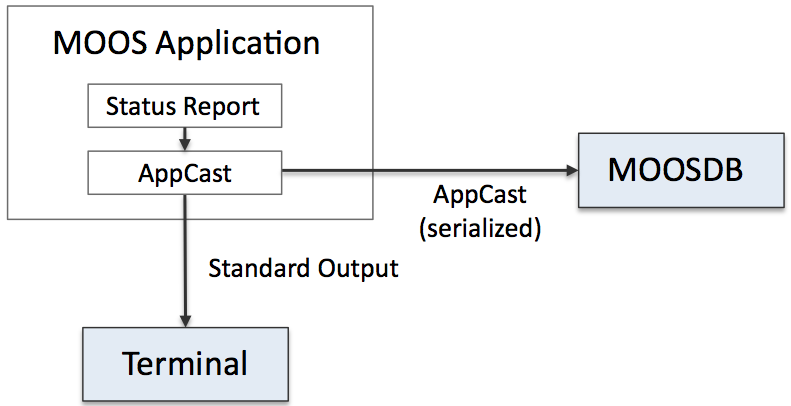
\includegraphics[width=0.5\textwidth]{figures/moos_withappcast.png}
  \end{minipage}
  \caption{An appcasting MOOS app produces terminal by repeatedly
    generating and sending an {\em appcast} to the terminal. The
    appcast is a also serialized and published to the MOOSDB for other
    MOOS applications to consume.}
\label{big_picture}
\end{figure}
\vspace{0.05in}


\newpage
%---------------------------------------------------------------------
\section{Overview of the pFooBar Interface and 
Configuration Options}

The \app{pFooBar} application may be configured with a
configuration block within a \var{.moos} file.
Its interface is defined by its publications and subscriptions
for MOOS variables consumed and generated by other MOOS
applications. An overview of the set of configuration options and
interface is provided in this section.

\subsection{Configuration Parameters of pFooBar}
\index{pFooBar!Configuration Parameters}
\index{Configuration Parameters!pFooBar}

The following parameters are defined for \app{pFooBar}. A more
detailed description is provided in other parts of this
section. Parameters having default values indicate so in parentheses
below.

\index{pFooBar!Configuration Parameters!\var{WATCH}}
\index{pFooBar!Configuration Parameters!\var{NOWATCH}}
\index{pFooBar!Configuration Parameters!\var{WATCH\_ALL}}
\index{pFooBar!Configuration Parameters!\var{POST\_MAPPING}}
\index{pFooBar!Configuration Parameters!\var{SUMMARY\_WAIT}}
\begin{table}[H]
\renewcommand{\arraystretch}{1.2}
\begin{minipage}[c]{1.0\textwidth}

  \begin{tabular}{rp{0.78\textwidth}} 
    
    \var{NOWATCH:} & A process or list of MOOS processes to {\em not } watch. \\

    \var{SUMMARY\_WAIT:} & A maximum amount of time between
    \var{PROC\_WATCH\_SUMMARY} postings (-1). \\

    \var{WATCH:} & A process or list of MOOS process to watch and report on. \\

    \var{WATCH\_ALL:} & If true, watch all processes that become known (true). \\

  \end{tabular}
\end{minipage}
\end{table}


\subsection{MOOS Variables Published by pFooBar}
\index{pFooBar!Publications}
\index{Publications!pFooBar}

The primary output of \app{pFooBar} to the MOOSDB is a summary
indicating whether or not certain other processes (MOOS apps) are
presently connected.

\index[vars]{\var{PROC\_WATCH\_SUMMARY}} 
\index[vars]{\var{PROC\_WATCH\_EVENT}} 
\index[vars]{\var{PROC\_WATCH\_FULL\_SUMMARY}} 
\begin{table}[H]
\renewcommand{\arraystretch}{1.2}
\begin{minipage}[c]{1.0\textwidth}
  \begin{tabular}{rp{0.72\textwidth}} 

    \var{PROC\_WATCH\_EVENT}: & A report indicating a particular process
    has been noted to be gone missing or noted to have (re)joined the list of
    active processes. \\

    \var{PROC\_WATCH\_FULL\_SUMMARY}: & A single string report for
    each process indicating how many times it has connected and
    disconnected from the MOOSDB. \\

    \var{PROC\_WATCH\_SUMMARY}: & A report listing all missing processes,
    or ``All Present'' if no processes are missing. \\

  \end{tabular}
\end{minipage}
\end{table}

The user may also configure \app{pFooBar} to make a posting
dedicated to a particular watched process. For example, with the
configuration \var{WATCH = pNodeReporter:PNR\_OK}, the status of this
process is conveyed in the MOOS variable \var{PNR\_OK}, set to either
\var{"true"} or \var{"false"} depending on whether or not it is
present.

\pskip

The variable name for any posted variable may be changed to a
different name with the \var{POST\_MAPPING} configuration
parameter. For example, \var{POST\_MAPPING = PROC\_WATCH\_EVENT,
  UPW\_EVENT} will result in events being posted under the
\var{UPW\_EVENT} variable rather than \var{PROC\_WATCH\_EVENT}
variable.


\subsection{MOOS Variables Subscribed for by pFooBar}
\index{pFooBar!Subscriptions}
\index{Subscriptions!pFooBar}

The following variable(s) will be subscribed for by \app{pFooBar}:

\index[vars]{\var{DB\_CLIENTS}} 
\begin{table}[H]
\renewcommand{\arraystretch}{1.2}
\begin{minipage}[c]{1.0\textwidth}
  \begin{tabular}{rp{0.72\textwidth}} 
    \var{DB\_CLIENTS}: & A comma-separated list of clients currently
    connected to the MOOSDB, generated by the MOOSDB process.
  \end{tabular}
\end{minipage}
\end{table}


\subsection{Command Line Usage of pFooBar}
\label{sec_pfb_cmdline}
\index{Command Line Usage!pFooBar}
\index{pFooBar!Command Line Usage}
\index{Configuration Parameters!pFooBar}
\index{pFooBar!Configuration Parameters}

The \app{pFooBar} application is typically launched as a part
of a batch of processes by pAntler, but may also be launched from the
command line by the user. The command line options may be shown by
typing \var{"pFooBar --help"}:

\refstepcounter{listing}
\vspace{0.1in}
\noindent {\em {Listing \arabic{listing} - Command line usage for the
pFooBar tool.}}
\label{pfb_usage}
\footnotesize
\begin{verbatim}
   0  Usage: pFooBar file.moos [OPTIONS]               
   1                                                         
   2  Options:                                               
   3    --alias=<ProcessName>                                
   4        Launch pFooBar with the given process      
   5        name rather than pFooBar.                  
   6    --example, -e                                        
   7        Display example MOOS configuration block         
   8    --help, -h                                           
   9        Display this help message.                       
  10    --version,-v                                         
  11        Display the release version of pFooBar.    
\end{verbatim}
\normalsize
 
\subsection{An Example MOOS Configuration Block}

As of MOOS-IvP Release 4.2, most if not all MOOS apps are implemented
to support the \var{-e} or \var{--example} command-line switches. To
see an example MOOS configuration block, enter the following from the
command-line:

\small
\begin{verbatim}
  $ pFooBar -e
\end{verbatim}
\normalsize
\vspace{0.05in}

\noindent
This will show the output shown in Listing \ref{pfb_econfig} below.

\refstepcounter{listing}
\vspace{0.25in}
\noindent {\em {Listing \arabic{listing} - Example configuration of the 
pFooBar application.}}
\label{pfb_econfig}
\footnotesize
\begin{verbatim}
   0  =============================================================== 
   1  pFooBar Example MOOS Configuration                        
   2  =============================================================== 
   3  
   4  ProcessConfig = pFooBar
   5  {                                                               
   6    AppTick   = 4                                                 
   7    CommsTick = 4                                                 
   8                                                                  
   9    WATCH_ALL = true                                              
  10                                                                  
  11    WATCH  = pNodeReporter 
  12    WATCH  = pHelmIvP                                             
  13                                                                  
  14    NOWATCH = uXMS*                                               
  15                                                                  
  16  }                                               
\end{verbatim}
\normalsize
 
%---------------------------------------------------------------------
\section{Using and Configuring pFooBar}
\label{sec_pfoobar_usage}

Use this section to go into greater detail on the application. For example
it may be good to explain just exactly how to configure the application's
configuration parameters, and what they really mean. Likewise with the 
variables subscribed and published.


\end{document}


